%%%%%%
%%%%%%%%%%%%%%%%%%%%%%%%
%
% $Author: Sudeshna Nanda $
% $Datum: 2025-01-07  $
%$Pfad:Users/Documents/ML23-06-Magic-Wand-with-an-Arduino-Nano-33-BLE-sense/report/Contents/en/Deployment.tex $
% $Version: 1.0 $
% $Short Description: Deployment of the magic wand$
%%%%%%%%%%%%%%%%%%%%%%%%


\chapter{Deployment}
\label{chapter 9}

Following the KDD process, this chapter intends to explain the major components for the implementation in the Board Arduino nano 33 BLE Sense to detect specific gestures. This chapter will primarily be substantiated by previously covered topics, the deployment phase. Along with these concepts, the behavior of the board and system are also verified. 

\section{Application Description}

The Magic Wand is project leveraging gesture recognition to provide intuitive and seamless control over devices. It uses the Arduino Nano 33 BLE Sense with built-in sensors (accelerometer, gyroscope, and microphone) and a TensorFlow Lite gesture recognition model.\cite{Daity:21} This system interprets user gestures and translates them into commands, unlocking a wide range of applications, such as:

\begin{itemize}
	\item \textbf{Home Automation:} Control lights, appliances, and other IoT devices.
	\item \textbf{Gaming and AR/VR:} Enhance interactive experiences through gesture-based controls.
	\item \textbf{Assistive Technology:} Empower individuals with disabilities to interact with devices.
	\item \textbf{Healthcare:} Enable gesture-based monitoring and control in rehabilitation.
	\item \textbf{Education:} Teach gesture recognition and machine learning fundamentals in classrooms.\cite{Daity:21}
\end{itemize}

\section{Structure}

The deployment structure of the Magic Wand involves several interconnected components:

\subsection{Hardware}
\begin{itemize}
	\item \textbf{Arduino Nano 33 BLE Sense:} Equipped with sensors for data collection.
	\item \textbf{Sensors:}
	\begin{itemize}
		\item The accelerometer enables significant motion detection (SMD), which recognizes large-scale movements. SMD can be used to activate specific device functions, such as waking the system from sleep mode or triggering predefined actions based on significant gestures.\cite{Zhou:2020}
		\item The STMicroelectronics LSM9DS1 gyroscope is a precision instrument for measuring angular velocity around the x, y, and z axes. With adaptable measurement ranges of ±245, ±500, and ±2000 degrees per second (dps), the gyroscope is highly versatile for various applications such as inertial navigation, robotics, and drone stabilization.\cite{St:2024}
		\item a magnetometer, the x, y, and z axes (Mx, My, Mz) typically delineate the three-dimensional space in which the magnetic field is being assessed. The x-axis typically corresponds to the horizontal component of the magnetic field, the y-axis signifies the vertical component, and the z-axis reflects the magnetic field strength \cite{Kostiainen:2023}.
	\end{itemize}
\end{itemize}

\subsection{Software}
\begin{itemize}
	\item TensorFlow Lite provides one of the most popular model optimization techniques is called quantization.\cite{tensorflowlite:2025}
	\item A trained gesture recognition model deployed on the Arduino Nano.
\end{itemize}

\subsection{Data Processing}
\begin{itemize}
	\item Captures real-time sensor data.
	\item Preprocesses data for gesture recognition.
\end{itemize}

\subsection{Output/Interface}
\begin{itemize}
	\item Visual feedback via serial monitor.
	\item Actuation of connected devices or systems.
\end{itemize}

\section{Idea}

The Magic Wand translates motion data into meaningful actions by:
\begin{enumerate}
	\item Capturing real-time motion signals through sensors.\cite{Anh:2009}
	\item Preprocessing data to extract relevant features.
	\item Feeding preprocessed data into a pre-trained ML model for classification.
	\item Producing accurate gesture predictions.
	\item Translating predictions into actionable commands for device control or feedback.
\end{enumerate}

\section{Flow Chart}

\subsection{Overall System Flow Chart}

\begin{center}
	\begin{tikzpicture}[node distance=2cm]
		\node (start) [startstop] {Start};
		\node (wait) [process, below of=start] {Wait for Movement};
		\node (detect) [process, below of=wait] {Detect Gesture};
		\node (preprocess) [process, below of=detect] {Preprocess Data};
		\node (predict) [process, below of=preprocess] {Predict Gesture};
		\node (accuracy) [decision, below of=predict] {Check Prediction Accuracy?};
		\node (action) [process, right of=accuracy, xshift=4cm] {Perform Action};
		\node (retry) [process, left of=accuracy, xshift=-4cm] {Retry Prediction};
		\node (end) [startstop, below of=accuracy, yshift=-2cm] {End};
		
		\draw [arrow] (start) -- (wait);
		\draw [arrow] (wait) -- (detect);
		\draw [arrow] (detect) -- (preprocess);
		\draw [arrow] (preprocess) -- (predict);
		\draw [arrow] (predict) -- (accuracy);
		\draw [arrow] (accuracy.east) -- node[anchor=south] {Yes} (action.west);
		\draw [arrow] (accuracy.west) -- node[anchor=south] {No} (retry.east);
		\draw [arrow] (action) |- (end);
		\draw [arrow] (retry) |- (predict);
	\end{tikzpicture}
\end{center}

\section{ML Pipeline}

The ML pipeline for deploying the Magic Wand involves the following steps:

\subsection{Step 1: Problem Definition}
\begin{itemize}
	\item Define the goal: Recognize hand gestures as specific commands.
	\item Input: Real-time sensor data from accelerometer and gyroscope.
	\item Output: Predicted gestures.
\end{itemize}

\subsection{Step 2: Data Collection}
\begin{itemize}
	\item Collect raw sensor data for gestures using the Arduino Nano 33 BLE Sense.
	\item Store data in a structured format (e.g., JSON or CSV) with labeled gestures.
\end{itemize}

\subsection{Step 3: Data Preprocessing}
\begin{itemize}
	\item Normalize sensor data to a consistent range.
	\item Extract meaningful features such as velocity and angular motion.
	\item Encode gesture labels numerically for model training.
\end{itemize}

\subsection{Step 4: Dataset Splitting}
\begin{itemize}
	\item Divide the data into:
	\begin{itemize}
		\item Training set: 70\%
		\item Validation set: 20\%
		\item Test set: 10\%
	\end{itemize}
\end{itemize}

\subsection{Step 5: Model Design}
\begin{itemize}
	\item Choose a lightweight ML model such as a Convolutional Neural Network (CNN) or Recurrent Neural Network (RNN) optimized for time-series data.
\end{itemize}

\subsection{Step 6: Model Training}
\begin{itemize}
	\item Train the model using the training dataset.
	\item Validate the model periodically to avoid overfitting.
	\item Save checkpoints for the best model.
\end{itemize}

\subsection{Step 7: Model Evaluation}
\begin{itemize}
	\item Test the model on unseen data (test set).
	\item Evaluate accuracy, precision, recall, and F1-score.
\end{itemize}

\subsection{Step 8: Model Optimization}
\begin{itemize}
	\item Convert the model to TensorFlow Lite format.
	\item Apply quantization techniques to reduce size and improve inference speed.
\end{itemize}

\subsection{Step 9: Deployment}
\begin{itemize}
	\item Convert the quantized TensorFlow Lite model into a C header file.
	\item Integrate the model into the Arduino IDE.
	\item Upload the model to the Arduino Nano 33 BLE Sense.
\end{itemize}

\subsection{Step 10: Testing and Debugging}
\begin{itemize}
	\item Test the system for real-time gesture recognition.
	\item Debug issues with sensor data, model inference, or device integration.
\end{itemize}

\subsection{Step 11: Deployment to Real-World Application}
\begin{itemize}
	\item Use the Magic Wand for controlling devices, providing feedback, or integrating into larger systems.
\end{itemize}

\section{TensorFlow Lite (TFLite)}
\subsection{Description}
TensorFlow Lite provides one of the most popular model optimization techniques is called quantization. Quantization used to reduce the precision of the model’s parameters such as weights and activation outputs into 8-bit integers.\cite{tensorflowlite:2025} By default, all weights parameters are 32-bit floating-point numbers. It enables to greatly reduce the model size as 8-bit integers occupy less memory than 32-bit floating-point numbers. Although these 8-bit representations can be less precise so it turns outs little degradation in the model accuracy. TFLite supports techniques like 8-bit quantization, making models smaller and faster to run, and includes optimizations for CPUs, GPUs, and specialized accelerators.\cite{tensorflowlite:2025}

\subsection{Code Example}
\begin{lstlisting}[language=Python, caption={Running Inference with a TensorFlow Lite Model in Python}, label={code:tflite-inference}, style=pythonstyle]
	import tensorflow as tf
	import numpy as np
	
	# Load the TensorFlow Lite model
	interpreter = tf.lite.Interpreter(model_path="model.tflite")
	interpreter.allocate_tensors()
	
	# Get input and output tensors
	input_details = interpreter.get_input_details()
	output_details = interpreter.get_output_details()
	
	# Create input data
	input_data = np.array([[1.0, 2.0, 3.0]])
	
	# Set the input tensor
	interpreter.set_tensor(input_details[0]['index'], input_data)
	
	# Run inference
	interpreter.invoke()
	
	# Retrieve the output
	output_data = interpreter.get_tensor(output_details[0]['index'])
	print("Model Output:", output_data)
\end{lstlisting}


\subsection{Use of TensorFlow Lite (TFLite) in the Magic Wand Project}
Quantization can take place during model training or after model training. Here we are referring to the quantization during model training as Quantization-aware training.\cite{tensorflowlite:2025}
LiteRT now supports converting weights to 8-bit precision as part of model conversion from TensorFlow GraphDefs to LiteRT's flat buffer format. Dynamic range quantization achieves a $4\times$ reduction in model size. In addition, TensorFlow Lite (TFLite) supports on-the-fly quantization and dequantization of activations to allow for:

\begin{itemize}
	\item Using quantized kernels for faster implementation when available.\cite{tensorflowlite:2025}
	\item Mixing of floating-point kernels with quantized kernels for different parts of the graph.
\end{itemize}

The activations are always stored in floating point. For operations that support quantized kernels, the activations are quantized to 8-bit precision dynamically prior to processing and are dequantized to floating point precision after processing. Depending on the model being converted, this can provide a speedup over pure floating-point computation.

In contrast to quantization-aware training, the weights are quantized \textit{post-training}, and the activations are quantized dynamically at inference in this method. Therefore, the model weights are not retrained to compensate for quantization-induced errors. It is important to check the accuracy of the quantized model to ensure that the degradation is acceptable.\cite{tensorflowlite:2025}

\begin{itemize}
	\item \textbf{Model Training and Conversion:}
	TFLite is utilized during the development phase to convert a pre-trained TensorFlow model (e.g., a gesture recognition model trained on accelerometer data) into a lightweight format. The conversion process includes techniques such as quantization, where model weights and activations are reduced from 32-bit floating-point numbers to 8-bit integers. This step ensures that the model is optimized for memory usage and inference speed, making it suitable for the microcontroller.\cite{tensorflowlite:2025}
	
	\item \textbf{Testing and Validation:}
	TFLite is used to validate the model on a desktop or mobile device by running inference on example inputs (e.g., accelerometer data) and verifying the output classifications (e.g., \textit{wing}, \textit{ring}, or \textit{slope}). This testing ensures that the model performs accurately before deployment.
	
	\item \textbf{Optimization for Edge Deployment:}
	Using TFLite tools, the model is fine-tuned and optimized to run efficiently on edge devices like the Arduino Nano 33 BLE Sense. Profiling and optimizations ensure that the deployed model meets the hardware constraints.\cite{tensorflowlite:2025}
\end{itemize}
a TensorFlow model to train a simple Convolutional Neural Network (CNN) on the CIFAR-10 image dataset. We then evaluate the model's accuracy and save it for further quantization.

\subsection{TensorFlow Model Code}
In order to quantize model, we need a trained TensorFlow model. So, let’s train a simple CNN model on cifar10 image dataset from scratch. And will compare model accuracy of original TensorFlow model and the converted model with quantization.\cite{tensorflowlite:2025}
\begin{lstlisting}[language=Python, caption=TensorFlow CNN Model for CIFAR-10,style=pythonstyle, label={lst:quantization} ]
	
	import tensorflow as tf
	from tensorflow.keras import datasets, layers, models
	import matplotlib.pyplot as plt
	import numpy as np
	
	# Check TensorFlow version
	tf.__version__
	
	# Load CIFAR-10 dataset
	(x_train, y_train), (x_test, y_test) = datasets.cifar10.load_data()
	# Normalize the data to range [0, 1]
	x_train, x_test = x_train / 255.0, x_test / 255.0
	
	# Define a simple CNN model
	model = models.Sequential([
	layers.Conv2D(32, (3, 3), activation='relu', input_shape=(32, 32, 3)),
	layers.MaxPooling2D((2, 2)),
	layers.Conv2D(64, (3, 3), activation='relu'),
	layers.MaxPooling2D((2, 2)),
	layers.Conv2D(64, (3, 3), activation='relu'),
	layers.Flatten(),
	layers.Dense(64, activation='relu'),
	layers.Dense(10)  # Output layer for 10 classes
	])
	# Compile the model
	model.compile(optimizer='adam',
	loss=tf.keras.losses.SparseCategoricalCrossentropy(from_logits=True),
	metrics=['accuracy'])
	
	# Train the model
	history = model.fit(x_train, y_train, epochs=10, validation_data=(x_test, y_test))
	
	# Evaluate model accuracy
	test_loss, test_acc = model.evaluate(x_test, y_test, verbose=2)
	print(f"Original Model Accuracy: {test_acc:.4f}")
	
	# Save the model
	model.save("cifar10_cnn.h5")
	
	\end{lstlisting}

\textbf{Float16 quantization} reduces the model size by quantizing the model’s weight parameters to float16 bit floating-point numbers for a minimal impact on accuracy and latency. This quantization technique significantly reduces the model size by half.\cite{tensorflowlite:2025}

We add float16 quantization of weights while convert model into TensorFlow Lite. First set the optimizations flag to default optimizations that quantize all fixed parameters such as weights. Then specify float16 is the supported type on the target platform:

By default converted model still considered input and output as a float data type. This quantization method only quantized weight parameters. However, activations are still stored in floating-point.
	\begin{lstlisting}[language=Python, caption=TensorFlow Quantization for Model Conversion,style=pythonstyle, label={lst:float_quantization}]
	
		import tensorflow as tf
	
		# Load the trained model
		model = tf.keras.models.load_model("cifar10_cnn.h5")
		
		### Float16 Quantization ###
		converter = tf.lite.TFLiteConverter.from_keras_model(model)
	
		# Set the optimization mode
		converter.optimizations = [tf.lite.Optimize.DEFAULT]
	
		# Set float16 as the supported type on the target platform
		converter.target_spec.supported_types = [tf.float16]
	
		# Convert and save the Float16 quantized model
		tflite_model_fp16 = converter.convert()
		with open("model_fp16.tflite", "wb") as f:
		f.write(tflite_model_fp16)
	
		print("Float16 Quantized Model Saved: model_fp16.tflite")
	
		### Dynamic Range Quantization ###
		converter = tf.lite.TFLiteConverter.from_keras_model(model)
	
		# Set the optimization mode for dynamic range quantization
		converter.optimizations = [tf.lite.Optimize.DEFAULT]
	
		# Convert and save the dynamically quantized model
		tflite_model_dynamic = converter.convert()
		with open("model_dynamic.tflite", "wb") as f:
		f.write(tflite_model_dynamic)
	
		print("Dynamic Range Quantized Model Saved: model_dynamic.tflite")
	
	\end{lstlisting}
	
	\subsection{Key Differences Between Float16 and Dynamic Range Quantization}
	
	\begin{table}[h!]
		\centering
		\begin{tabular}{|l|l|l|}
			\hline
			\textbf{Feature} & \textbf{Float16 Quantization} & \textbf{Dynamic Range Quantization} \\
			\hline
			\textbf{Weight Precision} & 16-bit floating point & 8-bit integer \\
			\hline
			\textbf{Activation Storage} & Float32 & Float32 \\
			\hline
			\textbf{Inference Speed} & Slightly improved & Faster than Float16 \\
			\hline
			\textbf{Model Size Reduction} & $\sim$2x & $\sim$4x \\
			\hline
		\end{tabular}
		\caption{Comparison between Float16 and Dynamic Range Quantization}
	\end{table}
	\textbf{Integer quantization}
	Microcontroller devices, Edge TPU performs an integer-based operation. So above generated TFLite model won’t compatible with integer-only hardware. To execute the TensorFlow model on integer-only hardware, we need to quantize all model parameters, input and output tensor to an integer.\cite{tensorflowlite:2025}
	
	The post-training integer quantization is an optimization technique that converts both model’s weights and activation outputs from 32-bit floating-point numbers to the nearest 8-bit fixed-point numbers. It also quantizes a model’s input/output data. That tends to smaller model size and increased inference speed which is most suitable to deploy TensorFlow model on low-powered devices such as microcontrollers. Sometimes, it is also called full integer quantization as it converts all model parameters such as weights and activations into 8-bit integer numbers.\cite{tensorflowlite:2025}
	
	To quantize the variable data such as a model’s input/output and intermediates between layers, we need to provide a RepresentativeDataset by supplying a set of input data in a generator function. This enables the converter to estimate a dynamic range for all the variable data.\cite{tensorflowlite:2025}
	
	Here, integer-based quantization must be required integer input and output tensor for compatibility. By default, the TensorFlow Lite Converter assign the model input and output tensor in a float. Applying a full integer quantization technique to convert a model into TFLite:

\begin{lstlisting}[language=Python, caption=Full Integer Quantization for TensorFlow Model,style=pythonstyle, label={lst:full_integer_quantization}]
	
	import tensorflow as tf
	import numpy as np
	
	# Load the trained model
	model = tf.keras.models.load_model("cifar10_cnn.h5")
	
	# Load and preprocess CIFAR-10 dataset for representative dataset generation
	(x_train, _), (_, _) = tf.keras.datasets.cifar10.load_data()
	x_train = x_train.astype(np.float32) / 255.0  # Normalize
	
	# Function to generate a representative dataset
	def representative_data_gen():
	for input_value in tf.data.Dataset.from_tensor_slices(x_train).batch(1).take(100):
	yield [input_value]
	
	### Full Integer Quantization ###
	converter = tf.lite.TFLiteConverter.from_keras_model(model)
	
	# Set optimization mode
	converter.optimizations = [tf.lite.Optimize.DEFAULT]
	
	# Pass the representative dataset to help with activation quantization
	converter.representative_dataset = representative_data_gen
	
	# Restrict supported operations to INT8
	converter.target_spec.supported_ops = [tf.lite.OpsSet.TFLITE_BUILTINS_INT8]
	
	# Ensure input/output tensors are in INT8 format
	converter.inference_input_type = tf.int8
	converter.inference_output_type = tf.int8
	
	# Convert and save the quantized model
	tflite_model_int8 = converter.convert()
	with open("model_int8.tflite", "wb") as f:
	f.write(tflite_model_int8)
	
	print("Full Integer Quantized Model Saved: model_int8.tflite")
	
\end{lstlisting}
\begin{table}[h!]
	\centering
	\begin{tabular}{|l|l|}
		\hline
		\textbf{Feature} & \textbf{Full Integer Quantization (INT8)} \\
		\hline
		\textbf{Weight Precision} & 8-bit integer \\
		\hline
		\textbf{Activation Storage} & 8-bit integer \\
		\hline
		\textbf{Inference Speed} & Highest (suitable for Edge TPU \& microcontrollers) \\
		\hline
		\textbf{Model Size Reduction} & $\sim$4x smaller than FP32 \\
		\hline
	\end{tabular}
	\caption{Key Benefits of Full Integer Quantization (INT8)}
\end{table}

Full Integer Quantization offers significant advantages in terms of reduced model size and faster inference, making it ideal for deployment on low-power microcontrollers and Edge TPU accelerators. This method quantizes all parameters (weights and activations) to 8-bit integers, optimizing the model for edge devices.\cite{tensorflowlite:2024}

\section{TensorFlow Lite Micro (TFLite Micro)}
\subsection{Description}
LiteRT for Microcontrollers is designed to run machine learning models on microcontrollers and other devices with only a few kilobytes of memory. The core runtime just fits in 16 KB on an Arm Cortex M3 and can run many basic models. It doesn't require operating system support, any standard C or C++ libraries, or dynamic memory allocation.\cite{Tensorflowlite:2024}

\subsection{Code Example}
\begin{lstlisting}[language=C++, caption={Integrating TensorFlow Lite with LSM9DS1 Sensor for Gesture Detection}, label={code:tflite-imu-setup}, style=bashstyle]
	#include <TensorFlowLite.h>
	#include <Wire.h>
	#include <LSM9DS1.h>
	
	// Include the generated model C array
	extern "C" {
		#include "model.cc"
	}
	
	// Initialize objects
	LSM9DS1 imu;
	tflite::MicroInterpreter* interpreter;
	tflite::Model* model;
	tflite::MicroAllocator* allocator;
	
	// TensorFlow Lite setup
	void setup() {
		Serial.begin(9600);
		Wire.begin();
		
		if (!imu.begin()) {
			Serial.println("Failed to initialize IMU sensor!");
			while (1);
		}
		
		model = tflite::GetModel(model_tflite);
		interpreter = tflite::MicroInterpreter(model, allocator, tflite::kTensorArenaSize);
		
		Serial.println("Setup complete!");
	}
	
	void loop() {
		imu.readAccel();
		float input_data[] = {imu.accelX(), imu.accelY(), imu.accelZ()};
		
		for (int i = 0; i < 3; i++) {
			interpreter->input(0)->data.f[i] = input_data[i];
		}
		
		interpreter->Invoke();
		float* output = interpreter->output(0)->data.f;
		
		Serial.println(output[0] > 0.5 ? "Gesture Class: 1" : "Gesture Class: 0");
		delay(500);
	}
\end{lstlisting}


\subsection{Use of TensorFlow Lite Micro (TFLite Micro) in the Magic Wand Project}
TensorFlow Lite Micro (TFLite Micro) is designed specifically for running machine learning models on microcontrollers.Its use in the Magic Wand project is detailed below:

\begin{itemize}
	\item \textbf{Real-Time Inference on Arduino Nano 33 BLE Sense:}
	TFLite Micro enables the deployment of the lightweight TFLite model on the Arduino Nano 33 BLE Sense. The model is converted into a \texttt{C} array during deployment and integrated into the Arduino firmware. Real-time sensor data from the LSM9DS1 (accelerometer, gyroscope, and magnetometer) is processed by the model for gesture classification.
	
	\item \textbf{Memory and Computational Efficiency:}
	TFLite Micro is optimized for devices with limited memory (e.g., 256 KB RAM) and processing power. It employs static memory allocation and int8 quantization to ensure smooth execution of the model.
	
	\item \textbf{Gesture Recognition Flow:}
	The system follows these steps:
	\begin{enumerate}
		\item \textbf{Input:} Real-time accelerometer data is captured in three dimensions (X, Y, Z).
		\item \textbf{Preprocessing:} The data is normalized and formatted to match the input requirements of the model.
		\item \textbf{Inference:} The TFLite Micro interpreter processes the input through the model, classifying the gesture as \textit{wing}, \textit{ring}, \textit{slope}, or \textit{unknown}.
		\item \textbf{Output:} Based on the classification, the Arduino controls LEDs or sends visual feedback via the serial monitor.
	\end{enumerate}
	
	\item \textbf{Interactivity and Deployment:}
	TFLite Micro ensures real-time interactivity, allowing the Arduino Nano 33 BLE Sense to respond immediately to gestures. The deployment process involves embedding the model and the TFLite Micro runtime into the Arduino program, creating a portable and efficient system.
\end{itemize}

\textbf{Supported Platforms}

LiteRT for Microcontrollers is written in C++ 17 and requires a 32-bit platform. It has been tested extensively with many processors based on the Arm Cortex-M Series architecture, and has been ported to other architectures including ESP32. The framework is available as an Arduino library. It can also generate projects for development environments such as Mbed. It is open source and can be included in any C++ 17 project \cite{Tensorflowlite:2024}.

The following development boards are supported:

\begin{itemize}
	\item Arduino Nano 33 BLE Sense
	\item SparkFun Edge
	\item STM32F746 Discovery kit
	\item Adafruit EdgeBadge
	\item Adafruit LiteRT for Microcontrollers Kit
	\item Adafruit Circuit Playground Bluefruit
	\item Espressif ESP32-DevKitC
	\item Espressif ESP-EYE
	\item Wio Terminal: ATSAMD51
	\item Himax WE-I Plus EVB Endpoint AI Development Board
	\item Synopsys DesignWare ARC EM Software Development Platform
	\item Sony Spresense
\end{itemize}

\textbf{Explore the Examples}

Each example application is on GitHub and has a \texttt{README.md} file that explains how it can be deployed to its supported platforms. Some examples also have end-to-end tutorials using a specific platform, as given below:

\begin{itemize}
	\item \textbf{Hello World} - Demonstrates the absolute basics of using LiteRT for Microcontrollers.
	\item \textbf{Tutorial using any supported device} - \textit{Micro speech} - Captures audio with a microphone to detect the words "yes" and "no".
	\item \textbf{Tutorial using SparkFun Edge}
	\item \textbf{Person detection} - Captures camera data with an image sensor to detect the presence or absence of a person.
\end{itemize}

\textbf{Workflow}

The following steps are required to deploy and run a TensorFlow model on a microcontroller:

\begin{enumerate}
	\item \textbf{Train a model:} Generate a small TensorFlow model that can fit your target device and contains supported operations.
	\item \textbf{Convert to a LiteRT model:} Use the LiteRT converter to convert the model.
	\item \textbf{Convert to a C byte array:} Use standard tools to store the model in a read-only program memory on the device.
	\item \textbf{Run inference on the device:} Use the C++ library to run inference and process the results.
\end{enumerate}

\textbf{Limitations}

LiteRT for Microcontrollers is designed for the specific constraints of microcontroller development. If you are working on more powerful devices (for example, an embedded Linux device like the Raspberry Pi), the standard LiteRT framework might be easier to integrate.\cite{Tensorflowlite:2024}

The following limitations should be considered:

\begin{itemize}
	\item Support for a limited subset of TensorFlow operations.
	\item Support for a limited set of devices.
	\item Low-level C++ API requiring manual memory management.
	\item On-device training is not supported.
\end{itemize}


\subsection{Comparison of TFLite and TFLite Micro in the Project}
\begin{table}[h!]
	\centering
	\begin{tabular}{|p{4cm}|p{5cm}|p{5cm}|}
		\hline
		\textbf{Aspect} & \textbf{TFLite} & \textbf{TFLite Micro} \\
		\hline
		Purpose & Optimizes models for mobile/edge devices. & Executes models on microcontrollers. \\
		\hline
		Use Case in Project & Model conversion, quantization, and testing on desktop. & Real-time inference on Arduino Nano 33 BLE Sense. \\
		\hline
		Key Features & High-performance library with additional overhead. & Extremely lightweight and microcontroller-friendly. \\
		\hline
		Programming Context & Python for training and testing. & C++ for microcontroller deployment. \\
		\hline
	\end{tabular}
	\caption{Comparison of TFLite and TFLite Micro in the Magic Wand Project.}
\end{table}


\section{Gesture Recognition}
As already extensively detailed, the project's main objective is to recognize the gestures. To fully understand its implications and usage surroundings, explaining how the project’s scope can be translated into multiple and more complex implementations is necessary. Currently, the board will target three gestures which are trained in the data model and give feedback on the response of these gestures.

\subsection{Software}
In the Previous Software description\ref{ArduinoIDE}, Installation steps have been explained comprehensively. In the following codes, some important libraries are shown, which will be required to build the software part of the project. The main packages are from the LSM9DS1 for gesture output detection and tensorflow lite for Microcontrollers to run the trained model\ref{Model}. 
\begin{lstlisting}[language=C++, caption={C++ Code for Initializing TensorFlow Lite on Arduino}, label={code:arduino-tensorflow-init}, style=bashstyle]
	#include <Arduino_LSM9DS1.h>
	#include <TensorFlowLite.h>
	#include "tensorflow/lite/micro/micro_error_reporter.h"
	#include "tensorflow/lite/micro/micro_interpreter.h"
	#include "tensorflow/lite/micro/micro_mutable_op_resolver.h"
	#include "tensorflow/lite/schema/schema_generated.h"
	#include "tensorflow/lite/version.h"
\end{lstlisting}

Here is the recap of the Tensorflow lite Micro packages used in the Arduino: 
\begin{itemize}
	\item micro\_mutable\_op\_resolver.h provides the operations used by the interpreter to run the model.
	\item micro\_error\_reporter.h outputs debug information.
	\item micro\_interpreter.h contains code to load and run models.
	\item schema\_generated.h contains the schema for the TensorFlow Lite FlatBuffer model file format.
	\item version.h provides versioning information for the TensorFlow Lite schema.
\end{itemize}

Upon uploading the modified sketch and trained model through Tensorflow Lite Micro and the Arduino IDE, the board Arduino Nano 33 BLE Sense should exhibit gesture recognition capabilities. The recognized gestures, including wings, rings, and slope, will be displayed in the Serial Monitor of the Arduino editor during the project stage.

\section{Configuration}
%%%%%%%%%%%%%%%%%%%%%%%%%%%%%%%
After successfully fitting and uploading the model onto the Arduino Nano 33 BLE Sense board, the device operates under typical environmental conditions. The project's success depends on clearly defining the environment and conditions necessary for proper functionality. Understanding the module's surroundings is crucial. In this application, the Arduino Nano 33 BLE Sense board is connected directly to the computer via a Micro-USB cable, as explained in the Hardware section \ref{BoardDescription}. This connection powers the device during operation and facilitates data exchange with the user, along with essential calibration parameters for image capturing.

\subsection{Code Structure in Program}

In our program, it consists 12 major files. These files are coded under the Arduino IDE Platform. 

\subsection{Magic\_Wand.ino - isMoving()}
\begin{lstlisting}[language=C++, caption={C++ Function to Detect Movement Based on Accelerometer Data}, label={code:movement-detection}, style=bashstyle]
	bool IsMoving() {
		// Look at the most recent accelerometer values.
		const float* input_data = model_input->data.f;
		const float last_x = input_data[input_length - 3];
		const float last_y = input_data[input_length - 2];
		const float last_z = input_data[input_length - 1];
		
		// Figure out the total amount of acceleration being felt by the device.
		const float last_x_squared = last_x * last_x;
		const float last_y_squared = last_y * last_y;
		const float last_z_squared = last_z * last_z;
		const float acceleration_magnitude =
		sqrtf(last_x_squared + last_y_squared + last_z_squared);
		
		// Acceleration is in milli-Gs, so normal gravity is 1,000 units.
		const float gravity = 1000.0f;
		
		// Subtract out gravity to get the actual movement magnitude.
		const float movement = acceleration_magnitude - gravity;
		
		// How much acceleration is needed before it's considered movement.
		const float movement_threshold = 40.0f;
		const bool is_moving = (movement > movement_threshold);
		
		return is_moving;
	}
\end{lstlisting}

Here is one of the main functions in the program main file \FILE{Magic\_Wand.ino}. The above code determines whether a device is in motion based on accelerometer data. The function extracts the latest accelerometer values for the x, y, and z axes, calculates the total acceleration magnitude, and then subtracts the assumed normal gravity (1,000 units) to obtain the actual movement magnitude. The threshold for considering movement is set at 40.0 units, and the function returns true if the calculated movement magnitude exceeds this threshold, indicating that the device is in motion; otherwise, it returns false. It is essential to note that the threshold value may be application-specific and may need adjustment based on the particular context in which this code is employed.

\subsection{Magic\_Wand.ino - RecognizeGestures()}
\begin{lstlisting}[language=C++, caption={Gesture Recognition Using a Pretrained Model in C++}, label={code:gesture-recognition}, style=bashstyle]
	// This is the regular function we run to recognize gestures from a pretrained
	// model.
	void RecognizeGestures() {
		const bool is_moving = IsMoving();
		
		// Static state used to control the capturing process.
		static int counter = 0;
		static enum {
			ePendingStillness,
			eInStillness,
			ePendingMovement,
			eRecordingGesture
		} state = ePendingStillness;
		static int still_found_time;
		static int gesture_start_time;
		// State machine that controls gathering user input.
		switch (state) {
			case ePendingStillness: {
				if (!is_moving) {
					still_found_time = counter;
					state = eInStillness;
				}
			} break;
			
			case eInStillness: {
				if (is_moving) {
					state = ePendingStillness;
				} else {
					const int duration = counter - still_found_time;
					if (duration > 25) {
						state = ePendingMovement;
					}
				}
			} break;
			
			case ePendingMovement: {
				if (is_moving) {
					state = eRecordingGesture;
					gesture_start_time = counter;
				}
			} break;
			
			case eRecordingGesture: {
				const int recording_time = 128;
				if ((counter - gesture_start_time) > recording_time) {
					// Run inference, and report any error.
					TfLiteStatus invoke_status = interpreter->Invoke();
					if (invoke_status != kTfLiteOk) {
						TF_LITE_REPORT_ERROR(error_reporter, "Invoke failed on index: %d\n",
						begin_index);
						return;
					}
					
					const float* prediction_scores = interpreter->output(0)->data.f;
					const int found_gesture = PredictGesture(prediction_scores);
					
					// Produce an output
					HandleOutput(error_reporter, found_gesture);
					
					state = ePendingStillness;
				}
			} break;
			
			default: {
				TF_LITE_REPORT_ERROR(error_reporter, "Logic error - unknown state");
			} break;
		}
		
		// Increment the timing counter.
		++counter;
	}
\end{lstlisting}

The above section would like to define a function named "RecognizeGestures" that implements a state machine to capture and recognize gestures based on accelerometer data using a pretrained model. 

\begin{itemize}
	
	\item \textbf{Initialization of State and Counter:}
	
	The function begins by initializing some static variables to control the capturing process. A counter keeps track of the number of times the function has been called, and the state is an enumeration representing the different states in the gesture recognition process.
	
	\item \textbf{Gesture Recognition State Machine:}
	
	The core of the function is a state machine that manages the gesture recognition process. It includes the following functions:
	
	\begin{itemize}\label{statemanagement}
		
		\item ePendingStillness: Waits for the device to become still.
		\item eInStillness: Monitors the duration of stillness and transitions to the pending movement state if the stillness persists.
		\item ePendingMovement: Waits for the device to start moving.
		\item eRecordingGesture: Records accelerometer data for a specified duration, runs inference using a TensorFlow Lite model and produces an output based on the recognized gesture.
		
	\end{itemize}
	
	\item \textbf{State Transitions:}
	The function transitions between states based on the current state and the status of motion detection (is\_moving):
	
	\begin{itemize}
		
		\item From ePendingStillness to eInStillness if the device becomes still.
		\item From eInStillness to ePendingMovement if stillness persists for a specified duration.
		\item From ePendingMovement to eRecordingGesture if the device starts moving.
		
	\end{itemize}
	\item \textbf{Gesture Recording and Inference:}
	When in the eRecordingGesture state, the function records accelerometer data for a fixed duration (recording\_time) and then performs inference using a TensorFlow Lite model (interpreter->Invoke()). The result is processed using the PredictGesture function.
	
	\item \textbf{Output Handling:}
	The recognized gesture is processed further using the HandleOutput function, and the state is transitioned back to ePendingStillness to wait for the next gesture.
	
	\item \textbf{Error Handling:}
	The code includes error handling, reporting an error if the state machine encounters an unknown state.
	
	\item \textbf{Counter Increment:}
	The counter is incremented at the end of each function call to keep track of the overall timing.
	
\end{itemize}

\subsection{Magic\_Wand.ino - CaptureGestureData()}
\begin{lstlisting}[language=C++, caption={Gesture Data Capture State Machine in C++}, label={code:capture-gesture-data}, style=bashstyle]
	void CaptureGestureData() {
		const bool is_moving = IsMoving();
		
		// Static state used to control the capturing process.
		static int counter = 0;
		static int gesture_count = 0;
		static enum {
			eStarting,
			ePendingStillness,
			eInStillness,
			ePendingMovement,
			eRecordingGesture
		} state = eStarting;
		static int still_found_time;
		static int gesture_start_time;
		static const char* next_gesture = nullptr;
		// State machine that controls gathering user input.
		switch (state) {
			case eStarting: {
				if (!next_gesture || (strcmp(next_gesture, "other") == 0)) {
					next_gesture = "wing";
				} else if (strcmp(next_gesture, "wing") == 0) {
					next_gesture = "ring";
				} else if (strcmp(next_gesture, "ring") == 0) {
					next_gesture = "slope";
				} else {
					next_gesture = "other";
				}
				TF_LITE_REPORT_ERROR(error_reporter, "# Hold the wand still");
				state = ePendingStillness;
			} break;
		}
	}
\end{lstlisting}

		The CaptureGestureData() function is to capture and process gesture data. This is crucial for the gesture recognition system within the interactive device. Key to its functionality are static variables and a boolean is\_moving variable, which together track the device's motion and gesture states. All these states have all mentioned earlier in the RecognizeGestures() function \ref{statemanagement}. The key difference is that it gathers training data and does not predict any gesture or record them. 
		
		\subsection{Magic\_Wand.ino - loop()}
	\begin{lstlisting}[language=C++, caption={Main Loop for Gesture Recognition or Data Capture}, label={code:loop-function}, style=bashstyle]
		void loop() {
			// Attempt to read new data from the accelerometer.
			bool got_data =
			ReadAccelerometer(error_reporter, model_input->data.f, input_length);
			const bool should_capture_data = false;
			if (should_capture_data) {
				CaptureGestureData();
			} else {
				RecognizeGestures();
			}
		}
	\end{lstlisting}
	
		
		The loop() function serves as the central operational loop for the program. It reads new data from the accelerometer to perform real-time motion tracking. The boolean got\_data indicates the success of this data acquisition. Intriguingly, the function includes a conditional should\_capture\_data, which, although set to false, suggests a dual-mode operation: one for capturing gesture data CaptureGestureData() and another for recognizing gestures RecognizeGestures(). Setting as false value can use the program in the prediction mode (i.e. RecognizeGestures()). 
		
		\subsection{Arduino\_acceleometer\_handler}
		\begin{lstlisting}[language=C++, caption={IMU Data Sampling and Buffer Management in C++}, label={code:imu-data-sampling}, style=bashstyle]
			while (IMU.accelerationAvailable()) {
				float x, y, z;
				// Read each sample, removing it from the device's FIFO buffer
				if (!IMU.readAcceleration(x, y, z)) {
					TF_LITE_REPORT_ERROR(error_reporter, "Failed to read data");
					break;
				}
				// Throw away this sample unless it's the nth
				if (sample_skip_counter != sample_every_n) {
					sample_skip_counter += 1;
					continue;
				}
				const float norm_x = -z;
				const float norm_y = y;
				const float norm_z = x;
				save_data[begin_index++] = norm_x * 1000;
				save_data[begin_index++] = norm_y * 1000;
				save_data[begin_index++] = norm_z * 1000;
				// Since we took a sample, reset the skip counter
				sample_skip_counter = 1;
				// If we reached the end of the circular buffer, reset
				if (begin_index >= 600) {
					begin_index = 0;
				}
				new_data = true;
			}
			
			// Skip this round if data is not ready yet
			if (!new_data) {
				return false;
			}
			
			// Check if we are ready for prediction or still pending more initial data
			if (pending_initial_data && begin_index >= 200) {
				pending_initial_data = false;
			}
			
			// Return if we don't have enough data
			if (pending_initial_data) {
				return false;
			}
			
			// Copy the requested number of bytes to the provided input tensor
			for (int i = 0; i < length; ++i) {
				int ring_array_index = begin_index + i - length;
				if (ring_array_index < 0) {
					ring_array_index += 600;
				}
				input[i] = save_data[ring_array_index];
			}
			return true;
		}
	\end{lstlisting}
	
	The Provided code offers a detailed illustration of efficient data acquisition, filtering, and preparation methodologies. Central to this process is the continuous monitoring of acceleration data availability, as evidenced by the while loop querying IMU.accelerationAvailable(). Upon successful data retrieval, indicated by IMU.readAcceleration(x, y, z), the code employs a strategic sampling approach, selectively processing every nth data point. This method, controlled by sample\_skip\_counter, effectively manages the data rate, a crucial aspect in scenarios with limited processing capabilities or specific data requirements. The transformation and normalization of the data into a different coordinate system, as seen in the assignment of norm\_x, norm\_y, and norm\_z, further exemplify the tailored preprocessing necessary for subsequent analytical stages.
	
	The implementation of a circular buffer, as indicated by the handling of begin\_index and the buffer size of 600, showcases an efficient data storage and management strategy, ensuring continuous data flow without overrunning memory limits. This approach is particularly relevant in real-time systems where older data is periodically replaced by newer inputs. The readiness of the data for further processing is meticulously managed through flags like new\_data and pending\_initial\_data, ensuring that the system only proceeds with sufficient data accumulation. 
	
	\subsection{Gesture\_Predictor}
	\begin{lstlisting}[language=C++, caption={Gesture Prediction Based on Model Output Scores}, label={code:gesture-prediction}, style=bashstyle]
		// Return the result of the last prediction
		// 0: wing("W"), 1: ring("O"), 2: slope("angle"), 3: unknown
		int PredictGesture(const float* prediction_scores) {
			int max_prediction_index = -1;
			float max_prediction_score = 0.0f;
			for (int i = 0; i < kGestureCount; i++) {
				const float prediction_score = prediction_scores[i];
				if ((max_prediction_index == -1) ||
				(prediction_score > max_prediction_score)) {
					max_prediction_score = prediction_score;
					max_prediction_index = i;
				}
			}
			
			int found_gesture;
			if ((max_prediction_index == kNoGesture) ||
			(max_prediction_score < kDetectionThreshold)) {
				found_gesture = kNoGesture;
			} else {
				found_gesture = max_prediction_index;
			}
			
			return found_gesture;
		}
	\end{lstlisting}
	
	
	The above code analyzes and predicts gestures based on an array of prediction scores. Each score in the array corresponds to a different gesture, and the function's role is to determine which gesture has the highest likelihood of being correct. It operates by iterating through the array of scores, returning numeric values 0, 1, 2 and
	3 for Wing, Ring, Slope and unknown respectively and maintaining a record of the highest score encountered and its associated index. This is achieved through a for-loop that compares each score with the current maximum; if a higher score is found, the function updates the maximum score and its corresponding index. 
	
	Initially the "prediction scores" obtained from the main is passed on to the function in which a "maxPredictionScore" and "maxPrediction Index". These values above are then compared to "kNoGesture" and "kDetectionThrehsold", then the value of found gesture variable is found which is equal to max prediction index. 
	
	\subsection{Arduino\_Output\_Handler}
\begin{lstlisting}[language=C++, caption={LED Control Based on Gesture Recognition}, label={code:led-control}, style=bashstyle]
	const int ledPinRed = 22;
	const int ledPinGreen = 23;
	const int ledPinBlue = 24;
	
	void LightUpRGB(int kind) {
		digitalWrite(ledPinRed, HIGH);
		digitalWrite(ledPinGreen, HIGH);
		digitalWrite(ledPinBlue, HIGH);
		
		switch (kind) {
			case 0: // W
			digitalWrite(ledPinRed, LOW);
			break;
			case 1: // O
			digitalWrite(ledPinGreen, LOW);
			break;
			case 2: // L
			digitalWrite(ledPinBlue, LOW);
			break;
			default:
			break;
		}
	}
	
	void HandleOutput(tflite::ErrorReporter* error_reporter, int kind) {
		// The first time this method runs, set up our LED
		static bool is_initialized = false;
		if (!is_initialized) {
			pinMode(LED_BUILTIN, OUTPUT);
			pinMode(ledPinRed, OUTPUT);
			pinMode(ledPinGreen, OUTPUT);
			pinMode(ledPinBlue, OUTPUT);
			is_initialized = true;
		}
		// Toggle the LED every time an inference is performed
		static int count = 0;
		++count;
		if (count & 1) {
			digitalWrite(LED_BUILTIN, HIGH);
		} else {
			digitalWrite(LED_BUILTIN, LOW);
		}
		
		LightUpRGB(kind);
	}
\end{lstlisting}

		
		\begin{itemize}
			\item \textbf{Variable Declarations:}
			"ledPinRed, ledPinGreen, ledPinBlue:" These are constants representing the pin numbers to which the red, green, and blue LEDs are connected. The values 22, 23, and 24 indicate the specific GPIO (General Purpose Input/Output) pins used.
			\item \textbf{Function LightUpRGB:}
			This function takes an integer kind as a parameter and controls the RGB LEDs based on the value of kind.
			Initially, it turns all LEDs (red, green, blue) on.
			The switch statement then determines which LED to turn off based on the value of kind (0 for red, 1 for green, 2 for blue).
			\item \textbf{HandleOutput:}
			This function is designed to handle the output based on an input kind.
			It initializes the LED pins only once, as indicated by the is\_initialized static variable.
			It toggles the built-in LED on the microcontroller on each call to indicate that an inference (or some processing) has been performed.
			Finally, it calls LightUpRGB(kind) to light up the appropriate LED based on the kind value.
		\end{itemize}
		
		Overall, this function serves as a state machine that captures accelerometer data, recognizes gestures using a pretrained TensorFlow Lite model, and handles the output based on the recognized gestures. The specific logic and parameters, such as stillness duration and recording time, can be adjusted based on the requirements of the application.
		
		\subsection{Upload the code to the board}
		Lastly, referring back to the Arduino IDE Configuration part\ref{uploadcode}, the program will be verified and uploaded to the board through the Arduino IDE. 
		
		\section{Tests}
		It is clear that after all the previous steps, some parameters need to be defined for the project functionality. This subsection’s objective is to present the result from the implementation on one part: SW. It is important to specify this feature to understand how the system will be under corroboration in the coming steps.
		
		\subsection{Common things to consider during Deployment test}
		The reliability of the neural network to recognize the digit increases with the increase in the training data. The neural network learns to abstract to the general rule and recognizes various aspects of the gestures, such as the speed of the movement and other factors.
		
		\subsection{Software tests}
		After creating Python programs for loading and processing images,
		it should be tested that the intended results are achieved. Also, after fitting the model, the performance of the CNN needs to be checked to see whether it is returning the desired results. Moreover, some negative test scenarios should be tested with the help of gestures apart from the wings, rings and slope.
		
		\section{Monitoring stage during deployment}
		%%%%%%%%%%%%%%%%%%%%%%%%%
		After the test, outputs from the board may not be accurate enough. At this moment, we should decide to modify the data set or add fresh training data. Therefore, we should monitor the model’s behavior to observe and record it. Alternatively, whenever a database suffers modifications due to environment changes, it is called Monitoring. The data set for this project is unchanged mainly because it only trains three gestures, and the remaining gestures are marked as unknown if they do not belong to the three trained gestures. In order to ensure that the model is robust enough since its first development, trained models may be changed to create several versions.
		
		The goal of this stage is to ensure that the knowledge extracted from the data is being used to make informed decisions and improve the system's overall performance. During this stage, the following activities are performed:
		
		\begin{itemize}
			\item \textbf{Performance monitoring:} This involves keeping a close eye on the effectiveness of the model created to interpret the data from the meters in order to make sure they are producing precise and pertinent findings.
			\item \textbf{Maintenance:} This entails maintaining the models and the database with fresh data and ensuring their functionality. In this particular case, since the database is "numbers," this is a very unusual case since numbers are universal.
			\item \textbf{Evaluation:} Finding any odd or unexpected trends in the meter data, such as	sudden spikes or dips in use, is a part of this process.
			\item \textbf{Feedback:} This involves setting up automated alerts or notifications to let consumers know when particular criteria are satisfied, such as when the use reaches a specific threshold or a leak is discovered.
			\item \textbf{Continuous improvement:} To enhance the performance of the models and the whole KDD process, this entails regularly monitoring the system and making the appropriate adjustments.
		\end{itemize}
		
		The KDD process can be enhanced over time by continuously monitoring the models and the data to spot any flaws, inconsistencies, or outliers in the data. It also gives the system’s users valuable insights to make better-educated decisions.
		
		
\chapter{Software Tests }
\label{chapter:SoftwareTests}

	The documentation for the magic wand project encompasses detailed explanations of each module, function, and class. It provides insights into the purpose, functionality, and importance of different components. The documentation also includes test classes and methods to ensure the correctness and reliability of the implemented functionalities. The clear organization of the project into modules promotes modularity and code maintainability.
	
	This comprehensive documentation serves as a valuable resource for project understanding, collaboration, and future development. It enhances transparency, allowing developers and stakeholders to grasp the project's architecture and functionality effectively.
	
	\section{Functions}
	
		\begin{itemize}
			
			\item \textbf{time\_wrapping(original\_data, factor, num\_frames)}
			
			The time\_wrapping function takes in an original\_data list, a time-wrapping factor, and the number of resulting num\_frames. It performs a time-wrapping operation on the input data, creating a modified dataset with a different temporal structure. This function is utilized in the data augmentation module to introduce temporal variations in the input data, contributing to the robustness of the trained model.
			
			\item \textbf{augment\_data(original\_data, original\_label)}
			
			The augment\_data function performs data augmentation by generating variations of the input original\_data and corresponding original\_label. It creates a more diverse dataset by applying operations such as time-wrapping. The augmented data is essential for improving the model's ability to generalize to various input scenarios.
			
			\item \textbf{setUp()}
			
			The setUp method is part of the test classes and is executed before each test case. It initializes necessary components for testing, such as data loaders or test-specific variables, ensuring a consistent and controlled environment for testing.
			
			\item \textbf{test\_time\_wrapping()}
			
			The test\_time\_wrapping method is a unit test for the time\_wrapping function. It checks whether the time-wrapping operation produces the expected number of frames and maintains the structure of the input data. This test ensures the correctness of the data augmentation technique.
			
			\item \textbf{test\_augment\_data()}
			
			The test\_augment\_data method is a unit test for the augment\_data function. It verifies that the augmented data has the expected length, type, and relationship with the original data and labels. This test is crucial to ensure the effectiveness of the data augmentation process.
			
		\end{itemize}
	
	\section{Classes}
	
		\begin{itemize}
		
		\item \textbf{TestAugmentation}
		
		The TestAugmentation class is a unittest class containing test methods for the data augmentation module. It tests the functionality of the data augmentation techniques, including time-wrapping and overall data augmentation.
		
		\item \textbf{TestLoad}
		
		The TestLoad class is a unittest class for testing the data loading module. It checks the correct initialization of data loaders and ensures that the loaded data has the expected structure and length.
		
		\item \textbf{TestPrepare}
		
		The TestPrepare class is a unittest class focusing on the correctness of the dataset preparation process. It tests functions related to preparing and writing data, including generating negative data to enhance dataset diversity.
		
		\item \textbf{TestSplit}
		
		The TestSplit class is a unittest class that validates the dataset splitting functionality. It ensures that the dataset is correctly split into training, validation, and testing sets according to specified ratios.
		
		\item \textbf{TestTrain}
		
		The TestTrain class is a unittest class dedicated to testing the model training process. It covers loading data, building neural network models (CNN and LSTM), and reshaping input data to ensure compatibility with the models.
		
		\end{itemize}
	
	\section{Test Files}
		
			\subsection{Unit Tests}
		
			One of the principles of \textbf{agile} development (although not exactly being the case for our study) is that testing should be tightly integrated with development, and programmers should write tests for their own code \cite{Ousterhout:2018}.
			
			\begin{itemize}
				\item unit tests
				\begin{itemize}
					\item most often written by developers
					\item small and focused
					\item are often run in conjunction with a test coverage tool\footnote{ensures that every line of code in the application is tested.}
					\begin{itemize}
						\item Coverage.py
						\item pytest-cov
					\end{itemize}
				\end{itemize}
			\end{itemize}
			
			When writing new code or modifying existing code, it is essential to update the corresponding unit tests to ensure continued code functionality and test coverage \cite{Ousterhout:2018}.
			
			Unit tests facilitate refactoring \cite{Ousterhout:2018}. Without a test suite
			
			\begin{itemize}
				\item It would be dangerous to make major structural changes to a system.
				\item bugs will go undetected until the new code is deployed.
				\begin{itemize}
					\item much more expensive to find and fix
				\end{itemize}
			\end{itemize}
			
			With a good set of tests, developers can be more confident when refactoring because the test suite will find most bugs that are introduced \cite{Ousterhout:2018}. 
			
			\subsection{\texttt{dataaugmentationtest.py}}
			
			This test code is responsible for verifying the functionality of the data augmentation process. Data augmentation involves creating variations of the existing dataset to enhance the model's ability to generalize. In the context of the magic wand project, it likely applies transformations to the gesture data such as rotation, scaling, or translation to create a more robust training set.
			
			To ensure that the data augmentation techniques are correctly implemented and producing the expected variations in the input data. This helps in improving the model's performance by exposing it to diverse examples of each gesture.
			
			\href{../Documents/MagicWand/ML23-06-Magic-Wand-with-an-Arduino-Nano-33-BLE-sense/Sourcecode/Code/Datatraining/Tests/dataaugmentationtest.py}{\texttt{dataaugmentationtest.py}}
		
			\begin{itemize}
				
				\item This test module validates the functionality of the data augmentation module used in the magic wand project. It specifically tests the \textbf{time\_wrapping} and \textbf{augment\_data} functions.
				 
				\item \textbf{test\_time\_wrapping}: Tests if the time wrapping function (time\_wrapping) produces the expected output dimensions and values.
				
				\item \textbf{test\_augment\_data}: Checks if the data augmentation function (\textbf{augment\_data}) appropriately increases the dataset size and maintains the correct structure.
				
			\end{itemize}
	
			\subsection{\texttt{dataloadtest.py}}
			
			This test code focuses on the loading of the dataset. It checks whether the dataset, which consists of gesture data (W, L, O), can be successfully loaded into the program. This includes reading image files, processing them, and organizing them for training or testing.
			
			To validate the functionality of the data loading process, ensuring that the code can access and organize the dataset correctly before feeding it into the machine learning model.
			
			\href{../Documents/MagicWand/ML23-06-Magic-Wand-with-an-Arduino-Nano-33-BLE-sense/Sourcecode/Code/Datatraining/Tests/dataloadtest.py}{\texttt{dataloadtest.py}}
			
			\begin{itemize}
				
				\item This module focuses on testing the data loading functionality of the project using the \textbf{DataLoader} class. It ensures that the training, validation, and test datasets are loaded correctly.
				
				\item \textbf{test\_get\_data:} Validates the structure and lengths of the loaded training, validation, and test datasets.
				
				\item \textbf{test\_pad:} Tests the padding functionality, ensuring it pads sequences correctly.
				
				\item \textbf{test\_format:} Verifies that the data is formatted as expected, and TensorFlow datasets are created.
				
			\end{itemize}
		
			\subsection{\texttt{datapreparetest.py}}
			
			The purpose of this test code is to verify the preparation of data before the training process. This may involve tasks such as normalization, resizing, or any other preprocessing steps required to make the data suitable for training.
			
			To confirm that the data is preprocessed correctly and is in the desired format for training the machine learning model.
			
			\href{../Documents/MagicWand/ML23-06-Magic-Wand-with-an-Arduino-Nano-33-BLE-sense/Sourcecode/Code/Datatraining/Tests/datapreparetest.py}{\texttt{datapreparetest.py}}
			
			\begin{itemize}
				
				\item This test module ensures the correctness of the dataset preparation process, including the creation of negative data and writing data to files.
				
				\item \textbf{test\_prepare\_data:} Checks if the original data is prepared correctly and matches the expected format.
				
				\item \textbf{test\_generate\_negative:} Verifies the generation of negative data.
				
				\item \textbf{test\_write\_data:} Tests if the data is correctly written to files and can be read back successfully.
				
			\end{itemize}
			
			\subsection{\texttt{datasplittest.py}}
			
			This test code is likely responsible for splitting the dataset into training, validation, and testing sets. It checks if the division is done correctly and ensures that each subset contains a representative distribution of the gestures.
			
			To guarantee that the dataset is appropriately divided, which is crucial for assessing the model's performance during training and testing phases.
			
			\href{../Documents/MagicWand/ML23-06-Magic-Wand-with-an-Arduino-Nano-33-BLE-sense/Sourcecode/Code/Datatraining/Tests/datasplittest.py}{\texttt{datasplittest.py}}
			
			\begin{itemize}
				
				\item This test module validates the dataset splitting functionality, ensuring that the data is divided into training, validation, and test sets as intended.
				
				\item \textbf{test\_read\_data:} Checks if the data is read correctly.
				
				\item \textbf{test\_split\_data:} Tests different scenarios of data splitting and verifies the lengths of the resulting datasets.
				
			\end{itemize}
			
			\subsection{\texttt{traintest.py}}
			
			The primary purpose of this test code is to validate the training process of the machine learning model. It includes setting up the model, feeding it with the training data, and monitoring its performance during training epochs.
			
			To ensure that the training process is functioning as expected, allowing the model to learn from the training data and adjust its parameters to make accurate predictions for the gestures.
			
			\href{../Documents/MagicWand/ML23-06-Magic-Wand-with-an-Arduino-Nano-33-BLE-sense/Sourcecode/Code/Datatraining/Tests/traintest.py}{\texttt{traintest.py}}
			
			\begin{itemize}
				
				\item This module focuses on testing the training process of the machine learning model. It includes building the neural network models, loading data, and reshaping the input.
				
				\item test\_load\_data: Validates the loading of training, validation, and test data as TensorFlow datasets.
				
				\item test\_build\_net: Tests the construction of CNN and LSTM models, ensuring the correct output shapes.
				
				\textbf{test\_reshape\_function:} Checks if the reshape function is correctly transforming the input data.
				
			\end{itemize}
			
			These test codes collectively contribute to the robustness and reliability of the magic wand project by validating different components of the machine learning pipeline.
		
		\section{Pytest Automation for Magic Wand Project Testing}
		
			Pytest is a testing framework that simplifies the process of writing and executing test code in Python. It allows you to create test functions, organize them into test modules, and run tests efficiently. Below is an overview of how you can use Pytest to automate the testing of your Magic Wand project.
			
			\subsection{Install Pytest}
			\begin{lstlisting}[language=Python, caption={Installing Pytest Using pip}, label={code:install-pytest}, style=pythonstyle]
				pip install pytest
			\end{lstlisting}
			
		
			\subsection{Folder Structure}
			
			Organize your test files into a folder named tests in your project directory. The file names should start with test to be discovered by pytest.
		
			\begin{verbatim}
				|-- magic_wand_project
				|-- Modules/
				|   |-- dataaugmentation.py
				|   |-- dataload.py
				|   |-- dataprepare.py
				|   |-- datasplit.py
				|   |-- train.py
				|-- Tests/
				|   |-- dataaugmentationtest.py
				|   |-- dataloadtest.py
				|   |-- datapreparetest.py
				|   |-- datasplittest.py
				|   |-- traintest.py
				|-- handleErrors/
				|   |-- errorHandler.py
			\end{verbatim}
		
			\subsection{Writing Test Functions}
			
			In each of your test files (e.g., dataaugmentationtest.py, dataloadtest.py, etc.), write test functions using the pytest naming convention (starting with test).
		
			\begin{lstlisting}[language=Python, caption={Example of Test Functions for Data Augmentation}, label={code:test-dataaugmentation}, style=pythonstyle]
				# Example: test_dataaugmentation.py
				
				def test_time_wrapping():
				# Test logic ...
				
				def test_augment_data():
				# Test logic ...
			\end{lstlisting}
			
			\subsection{Run Tests with Pytest}
			
			Open a terminal in the project directory and run:
			
			\textbf{pytest}
			
			pytest will automatically discover and execute all the test functions in the tests directory.
			
			\begin{itemize}
				
				\item \textbf{Pytest Command-Line Options}
				
				\begin{itemize}
					
					\item Run specific test file:
				
					\begin{lstlisting}[language=Python, caption={Running a Test for Data Augmentation with Pytest}, label={code:run-dataaugmentation-test}, style=pythonstyle]
						pytest tests/dataaugmentationtest.py
					\end{lstlisting}
					
					\item Run specific test function in a file:
				
					\begin{lstlisting}[language=Python, caption={Running a Specific Test with Pytest}, label={code:run-specific-test}, style=pythonstyle]
						pytest tests/dataaugmentationtest.py::test_time_wrapping
					\end{lstlisting}
					
					\item Show detailed output:
					
				\begin{lstlisting}[language=Python, caption={Running Pytest with Verbose Output}, label={code:run-pytest-verbose}, style=pythonstyle]
					pytest -v
				\end{lstlisting}
				
			
				\end{itemize}
		
				\item \textbf{Automation Script}
				
				To run all the tests together, you can create a simple automation script. For example, create a file named run\_tests.sh:
				
			\begin{lstlisting}[language=Python, caption={Bash Script for Running Pytest in a Specific Directory}, label={code:run-pytest-bash}, style=pythonstyle]
				#!/bin/bash
				
				# Navigate to the project directory
				cd Documents/MagicWand/
				ML23-06-Magic-Wand-with-an-Arduino-Nano-33-BLE-sense/
				Sourcecode/Code/Datatraining
				
				# Activate virtual environment if needed
				# source venv/bin/activate
				
				# Run pytest
				pytest
			\end{lstlisting}
			
				
				\item \textbf{Make the script executable}
				
			\begin{lstlisting}[language=Bash, caption={Setting Executable Permission and Running the Script}, label={code:set-permission-and-run}, style=bashstyle]
				chmod +x run_tests.sh
				
				# Run the script
				./run_tests.sh
			\end{lstlisting}
			
			\end{itemize}
	\subsection{Execution}
	
	The result of running \texttt{pytest} in the \texttt{Command Prompt} in the directory of the test files is shown in Figure \ref{fig:pytestResult}.
	
	\begin{figure}[h!]
		\centering
		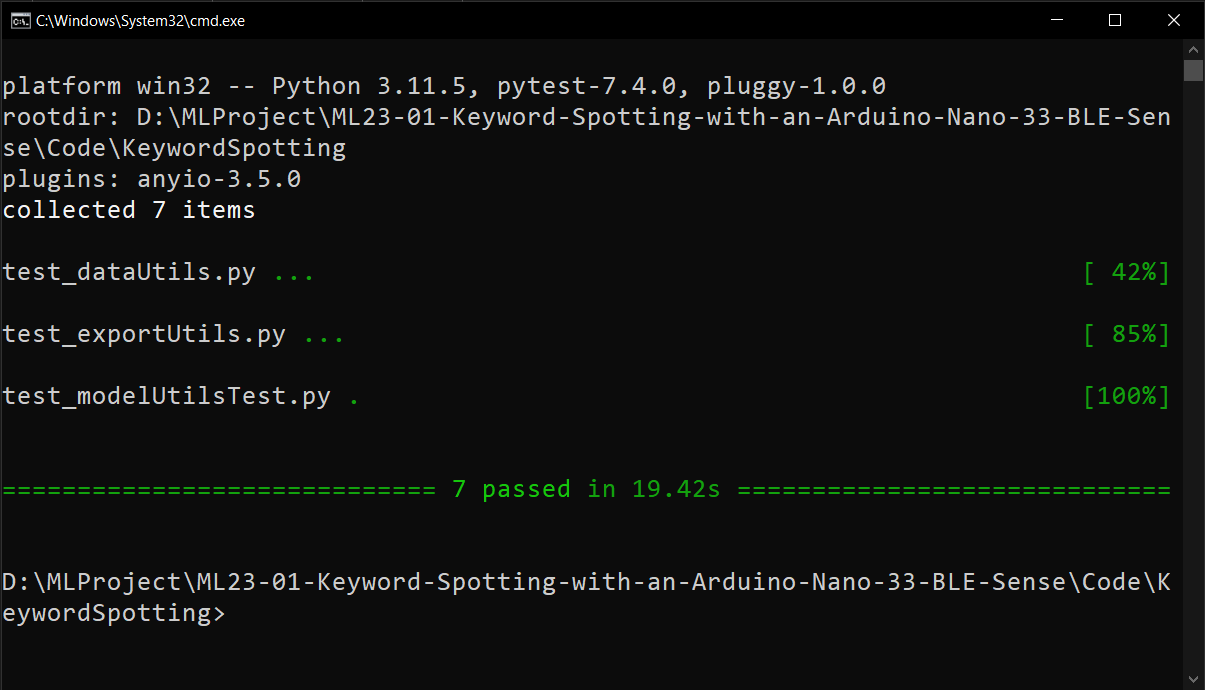
\includegraphics[width=100mm]{Images/Programming/pytestResult}
		\caption{Result of running \texttt{pytest} in the direcotry of the test files in \texttt{Command Prompt}} 
		\label{fig:pytestResult}
	\end{figure}
	
	\begin{verbatim}
		collected 7 items
	\end{verbatim}
	
	This line indicates that \texttt{pytest} found and collected a total of 7 test items. These items represent individual test files or modules in the project. Note that the name of the files has been changed, starting with "\texttt{test\_}" so that \texttt{pytest} could automatically find them.
	
	\begin{verbatim}
		test_dataUtils.py ...                      [ 42%]
		test_exportUtils.py ...                    [ 85%]
		test_modelUtilst.py .                      [100%]
	\end{verbatim}
	
	Each line corresponds to the progress of test execution for a specific test file. Dots (\texttt{...} and \texttt{.}) represent successful tests. For the case of \texttt{...}, three tests were successful, each dot representing a successful test. The percentage values ([42\%], [85\%], [100\%]) indicate the progress through the entire test suite.
	
	\begin{verbatim}
		7 passed in 28.32s 
	\end{verbatim}
	
	This final summary line provides an overview of the test results. It states that out of the 7 tests executed, all 7 passed successfully. The total execution time for all tests was 28.32 seconds. The [100\%] success rate indicates that all the tests you ran have passed.